\documentclass[12pt]{article}
\usepackage{fullpage}
\usepackage{latexsym}
%\usepackage[utf8]{inputenc}
%\usepackage[T1]{fontenc}
\usepackage[danish,english]{babel}
\usepackage{amsmath}
\usepackage{amsfonts}
\usepackage{amssymb}
\usepackage{amsthm}
\usepackage{graphicx}
\usepackage{float}
\usepackage[ampersand]{easylist}
\usepackage{caption}
%%\usepackage{subcaption}
\usepackage{epstopdf}
\usepackage[format=hang,font=small]{caption} 	% Pretty captions
\usepackage{wrapfig} 
\usepackage{lscape}
\usepackage{subfig}
\usepackage{booktabs}
\usepackage{xcolor}
\usepackage{bbold}
\numberwithin{equation}{section}
\newcommand{\norm}[1]{\left\lVert #1 \right\rVert}
\newcommand{\avg}[1]{\left< #1 \right>}
\newcommand{\ket}[1]{\left| #1 \right\rangle}
\newcommand{\bra}[1]{\langle\left. #1 \right|}
\newcommand{\dprod}[2]{\langle #1 | #2 \rangle}
\newcommand{\Ohat}{\hat{\mathcal{O}}}
\newcommand{\fv}[1]{\mathbf{#1}}
\newcommand{\fp}{\mathbf{P}}
\newcommand{\pdif}[1]{\frac{\partial}{\partial #1}}
\newcommand{\rdif}[1]{\frac{d}{d #1}}
\newcommand{\cop}{c_{\uparrow}^{\phantom{\dagger}}}
\newcommand{\copd}{c_\uparrow^{\dagger}}
\newcommand{\cdown}{c_{\downarrow}^{\phantom{\dagger}}}
\newcommand{\cdownd}{c_\downarrow^\dagger}
\newcommand{\rref}[1]{(\ref{#1})}
\renewcommand{\v}[1]{\ensuremath{\mathbf{#1}}} % for vectors
\newcommand{\gv}[1]{\ensuremath{\mbox{\boldmath$ #1 $}}} % for vectors of Greek letter
\newcommand{\dint}[1]{\, \mathrm{d }#1}
\newcommand{\dintc}[1]{\mathrm{d} #1 \,} % For beautiful integration variable declaration such as dx
\newcommand{\sgn}{\mathrm{sgn}}
\newcommand{\matr}[1]{\underline{\underline{#1}}}
\newcommand{\A}{\mathcal{A}}
\usepackage{ulem}
\begin{document}
\title{Cellular Automata}
\author{Fysikklubben}
\maketitle
\begin{enumerate}
\item Definition, examples in 1 and 2D.
\item Properties
\subitem Pretty Pictures
\subitem Universal Computing
\subitem Modelling of physical, chemical, biological and social systems
\item Example model: Game of Life
\item Example model: The neuron model
\item Example model: reaction-diffusion model
\item Comments on Fredkin's Finite Nature
\end{enumerate}




\section{Introduction}
Cellular Automata are dynamical systems in d dimensions with discrete time steps. The system consists of "cells" which are located in some lattice (or, in general, cells sit on nodes in a graph). Each cell can be found in some number, \(k\), of different states. Often, when we try to model some specific system or mimic some effect in the world, the states naturally correspond to "physical states", e.g. we may have two states: "Dead" and "Alive" or three: "Inhibited", "Excited", "Firing", depending on the application. The update rules are local, meaning that the state of cell \(i\) at time \(t\) depends on the state of neighbouring cells at time \(t-1, t-2, ..., t-\ell\) for some finite \(\ell\), which is called the "order" of the model. A theory with a given neighbourhood (defined in some way), a number of states per cell and an update-rule is called a Cellular Automaton. The restriction of locality in time and space implies that there are a finite number of possible cellular automata, but of course we may vary initial conditions, change the number of states per cell, change the definition of "neighbourhood", and change the order of the theory. This leads to an incredibly rich menagerie of automata - but in fact even deceivingly simple 1-D cellular automata display complex behaviour. 

Let's look at 1D automata to begin with.


\paragraph{1D Cellular Automata}
Let us assume that the neighbourhood for a cell is always symmetrical. Then there are only three parameters to worry about: the number of neighbours, i.e. the size of the neighbourhood, the order of the system and the number of states per cell. Let us consider a first order system with three neighbours (which includes the cell itself) with two states (0 and 1) per cell. In this case there are \(2^3\) possible configurations of any given neighbourhood, and for each of these we must determine how the central cell evolves. Since there are two choices for the central cell per neighbourhood state we find \(2^{2^3} = 256\) possible update-rules/cellular automata. We can order the possible neighbourhood states in some arbitrary way, and then indicate a given automaton by a string of 1s and 0s. As an example, the automaton in figure \ref{RandomCA} is given by the string \(10010110\). Interpreting this a number in base 2 yields an enumeration of all the possible 1D, first order, k = 3 Cellular Automata. 

\begin{figure}[H]
\centering
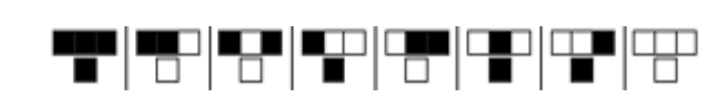
\includegraphics[width=0.8\textwidth]{RandomCA.png}
\caption{}
\label{RandomCA}
\end{figure}

I will not go through all 256 of these. They show varied behaviour ranging from trivial (e.g. rule 0) to periodic, to random, to somewhere in between periodicity and randomness (e.g. chaotic or complex CA). Before we move on, let me mention rule 110 = \(01101110\) (base 2). This falls in the class of complex automata. Starting from one cell in state 1 (coloured black) we find the evolution shown in figure \ref{rule110}
\begin{figure}[H]
\centering
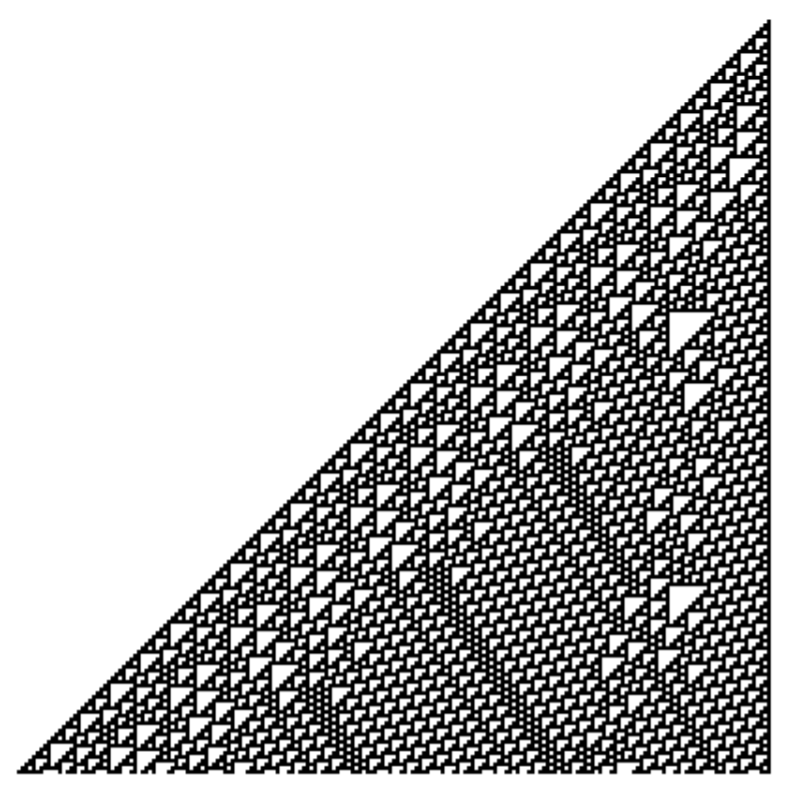
\includegraphics[width=0.8\textwidth]{rule110.png}
\caption{}
\label{rule110}
\end{figure}    
We see complex, seemingly random triangular patterns. Compare with this sea-shell:
\begin{figure}[H]
\centering
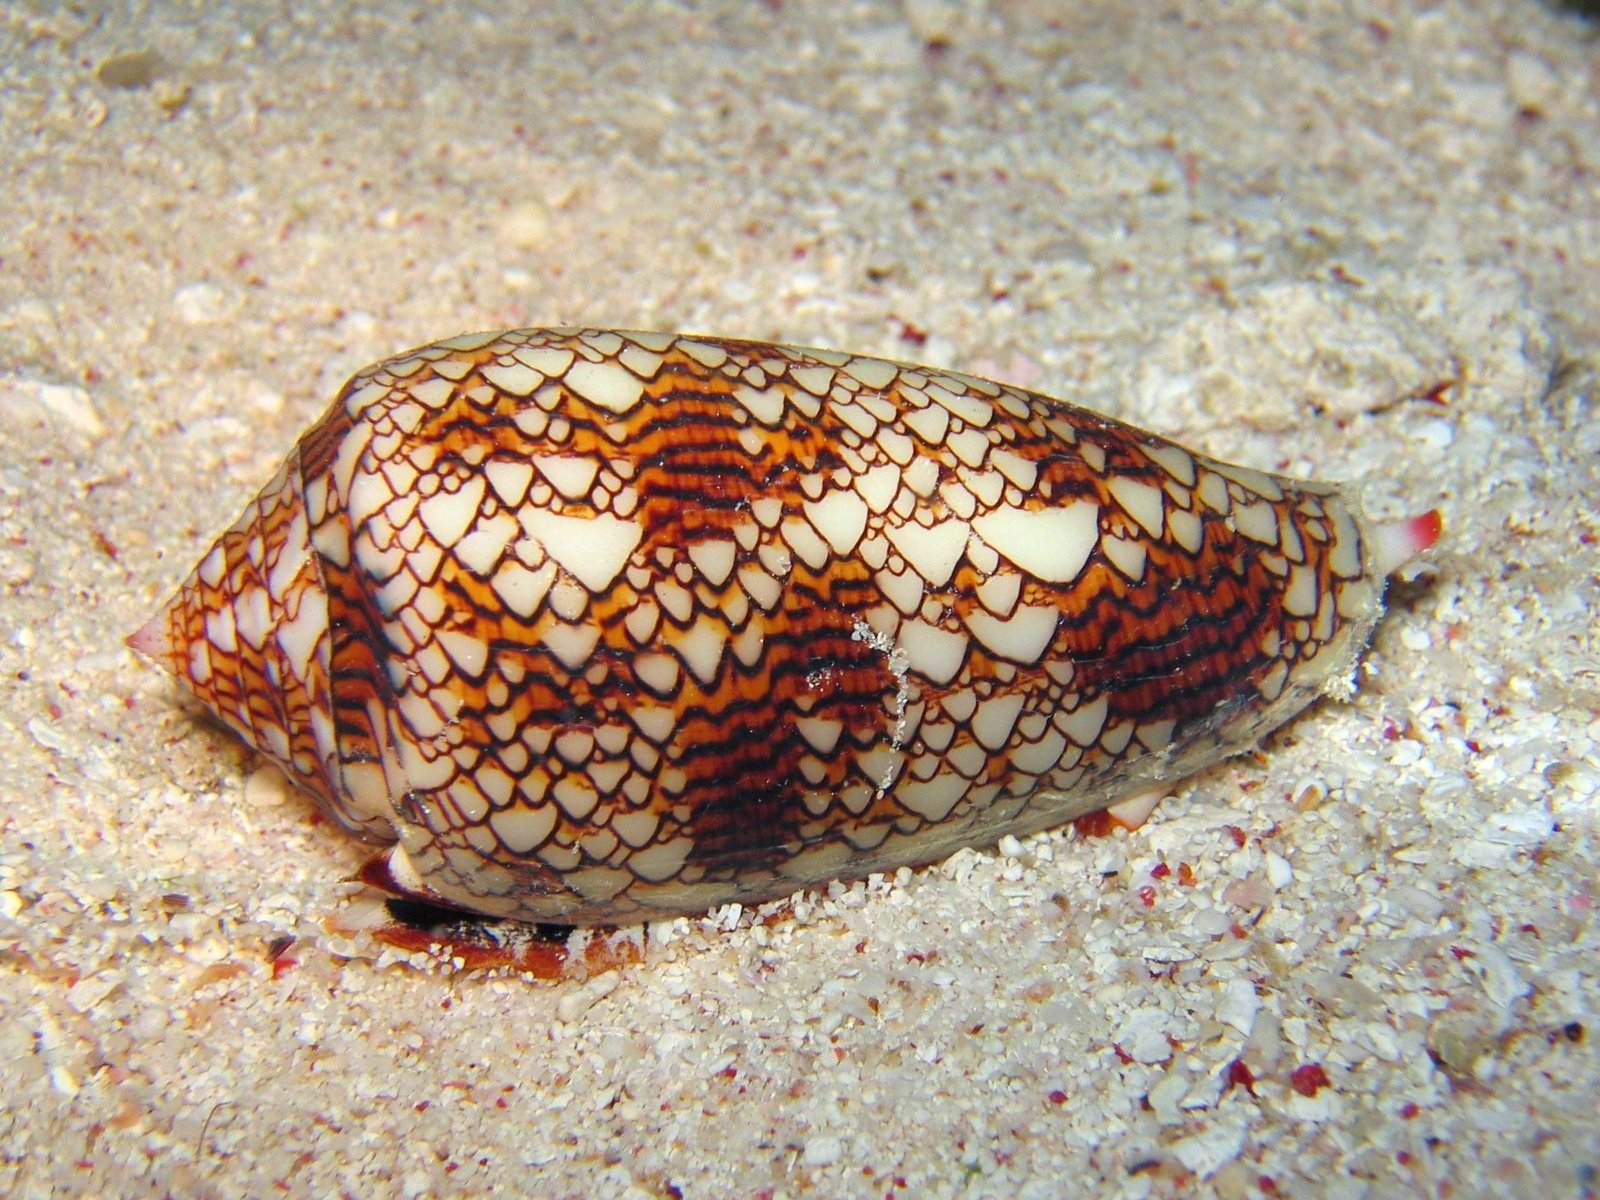
\includegraphics[width=0.8\textwidth]{Seashell.jpg}
\caption{}
\label{Seashell}
\end{figure}    

It turns out that these deceptively simple systems can display exceedingly complex behaviour on large scales. This makes them interesting objects of study for a number of reasons.

\subsection{Some properties of Cellular Automata}
Because of the complexity they display, automata have found use in fields ranging from physics to economics. Clearly, they can be considered as simple toy models used to explore emergent phenonema in many-body systems. Researchers have had succes in describing characteristic features of galaxy formation, pigmentation in animals, segregation of cities and the dynamics of chemical reactions.

However, the complexity of cellular automata make them interesting in their own right. One can study such things as the statistical mechanics, dynamical properties and computational complexity of automata. In fact, certain automata have been found to be \textit{universal computers} meaning they can perform any computation that is possible to perform - that is, these cellular automata are capable of as complex and varied behaviour as any computer. Rule 110 above is an example of such a universal computer. Stephen Wolfram postulates that the automata capable of universal computation are exactly the ones that are chaotic. An interesting notion.

The final reason (I can think of) why one might be interested in cellular automata is that they (sometimes) produce pretty pictures.
\begin{figure}[H]
\centering
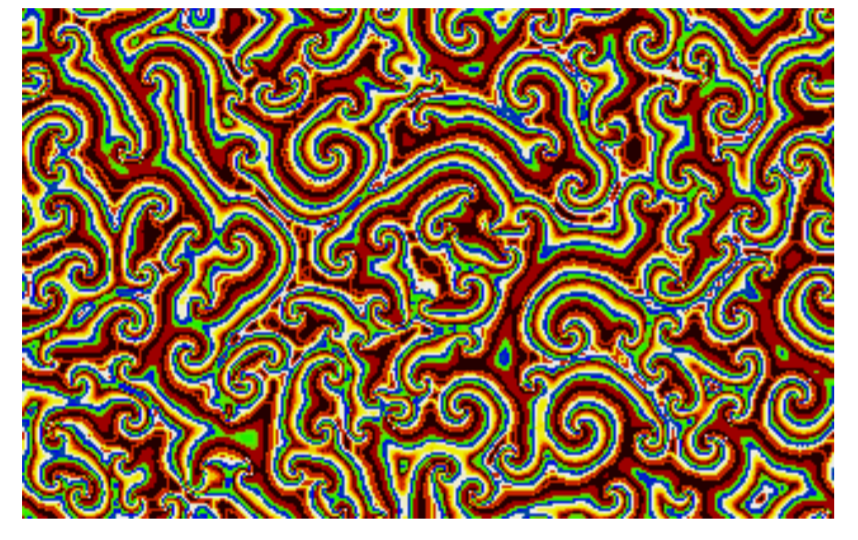
\includegraphics[width=0.8\textwidth]{HodgepodgeMachine.png}
\caption{The hodgepodge machine.}
\label{HodgepodgeMachine}
\end{figure}  



\section{Examples}
\subsection{Game of Life}
Probably the most well-known cellular automaton is Conway's Game of Life. The cells can be in one of two states: "Dead" or "Alive". The cells live on a 2D grid and the state of a cell at the next time-step depends on the state of its 8 closest neighbours at the current time-step. The update rule is the following:
\begin{enumerate}
\item Any cell with 1 or 0 living neighbours dies
\item Any living cell with 2 or 3 neighbours lives
\item Any dead cell with exactly 3 neighbours becomes alive
\item Any cell with more than three neighbours dies
\end{enumerate}
Despite the fact that the state-space and rules are quite simple this automaton shows really complex behaviour. There are indefinitely stable "Lifeforms", Lifeforms that reproduce in a certain sense and there are many complex, periodic Lifeforms known. In fact, the Game of Life is capable of universal computing. I will only give two examples and no code because it is very easy to find both online.
\begin{figure}[H]
\centering
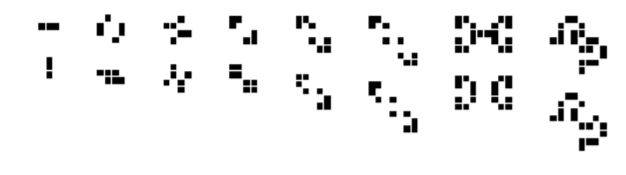
\includegraphics[width=0.8\textwidth]{GOLPeriod2.png}
\caption{A bunch of period 2 Lifeforms.}
\label{GOL2}
\end{figure}  
\begin{figure}[H]
\centering
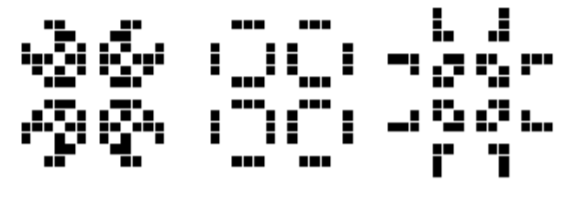
\includegraphics[width=0.8\textwidth]{GOLPeriod3.png}
\caption{A period 3 Lifeform.}
\label{GOL3}
\end{figure}  


\subsection{The Neuron Model}
\paragraph{Introduction \\}
The next model we will talk about is due to Pytte. State of the art methods for describing neural systems involve huge numbers of differential equations, e.g. for 10,000 neurons one must solve 250,000 coupled differential equations. The reason for this complexity is that the mathematical description attempts to describe the underlying physical system very accurately: one accounts for currents in and connectivities of the axons connected to each neuron. In this kind of situation a cellular automaton is interesting for two reasons. Cellular automata are generally much faster to simulate than a differential equation description of the same system, so if one can find a CA that describes the system "well" one can perform (maybe preliminary) analyses much faster. Secondly, simplification is interesting in its own right, since it may allow one to single out the features of the system that produce characteristic phenomena. This can often provide a better understanding of the fundamental principles that are in play.

Pytte's CA attempts to model the hippocampi which are regions of the brain that are critical to the formation of memories and in spatial navigation. A lot of experimental data is apparently available on the hippocampi. I do not know how many of the features of Pytte's model are specific to the hippocampi and how many are generally applicable to neural systems. With that disclaimer, let us begin.

\paragraph{CA Hippocampus\\}
There are three types of neurons in our model: excitatory (e), fast inhibitory (f), and slow inhibitory (s). Each neuron is a two-state system: "resting" and "firing". We specifiy the number of each type of neuron, and the number of other neurons each type is connected to. These connections are distributed randomly. The connections are directed, meaning the signal only travels in one direction along the connection. This means this CA lives on a general directed graph and we don't really have a notion of spatial dimension. We assume that each neural connection has a "bond strength" which is determined by the neuron from which the connection originates. Bond strengths are given by \(K_e, K_f, K_s\).

Even though each neuron is either firing or not, because propagation along axons is not instantaneous, neurons fire for some period of time and because neurons may spontaneously fire we need to include extra automaton states to account for these effects.

Signals from excitatory neurons to inhibitory neurons are the fastest, so here we assume no latency; if (e) is firing at time \(t\) then connected inhibitory neurons feel this effect at the next time-step. For other connections we introduce latencies \(\tau_e, \tau_f, \tau_s\). \(\tau_q\) is the latency for signals to propagate from a neuron of type \(q\) to an excitatory neuron. Inhibitory neurons are not affected by other inhibitory neurons so we do not need to consider such connections.

Additionally, each type of neuron fires for some amount of time. In brains the slow inhibitory neurons fire considerably longer than the other types. We indicate the length of the firing times by \(\varphi_q\) for a neuron of type \(q\).

Only excitatory neurons fire spontaneously. The time before spontaneneous firing is \(\sigma\); this number is random and different for each neuron.

Finally the excitatory neurons have a refractory period given by \(\rho\). 

The states of the excitatory neurons consists of several pieces of data: the current state (resting or firing), the time since last fired (for excitatory neurons) and the spontanteneous firing time. This last datum does not change under time-evolution but is generally different for each neuron. For inhibitory neurons we do not need the last two pieces of data. 
\begin{align}
(e): & \underbrace{0}_{resting}, \underbrace{1, 2, ..., \varphi_e}_{firing}; \; \; \alpha; \; \; \sigma, \\
(q): & \underbrace{0}_{resting}, \underbrace{1, 2, ..., \varphi_q}_{firing}. 
\end{align}
Note also that because of the latency effects we have to store the states for a time \(\max\{\tau_e,\tau_f,\tau_s\} \; (=\tau_s)\). 
%\begin{align}
%(e):& \underbrace{0, 1, 2, ..., \sigma}_{resting}, \underbrace{\sigma+1,\sigma+2,..., \sigma+ \tau_e}_{firing; \; delay\;period}, \underbrace{\sigma+ \tau_e+1, ..., \sigma+\tau_e + \varphi_e}_{firing; \;active}, \nonumber \\
%&\underbrace{\sigma+\tau_e+\varphi_e+1, ... \sigma+\tau_e+\varphi_e+\rho}_{refractory\,period}, \\
%(q):& \underbrace{0}_{resting}, \underbrace{1, 2, ... , \tau_d^q, \tau_d^q}_{firing; \; delay \; period}, \underbrace{\tau_q + 1, ..., \tau_q+\varphi_q}_{firing; \; active} \;\; q = f,s.
%\end{align}
The update rules are as follows:
\begin{align}
(e): \;& \alpha \rightarrow \alpha +1, && \mathrm{if} \; S = 0, \\
& \alpha = 1, &&\mathrm{if} \; S \neq 0, \\
& 0 \rightarrow 1, && \mathrm{if} \; m_e(t) K_e -(m_f(t)K_f+m_s(t)K_s) > h(S(t)), \\
& 0 \rightarrow 1, && \mathrm{if} \; \alpha \geq \sigma, \\
& S \rightarrow S +1, && \mathrm{if} \; S>0.
\end{align}
Here \(m_q(t)\) counts the number of connected, firing neurons of type \(q\) at time \(t-\tau_q\), and
\begin{align}
h(S(t)) =\begin{cases} F(\rho-\alpha)/\rho & \alpha \leq \rho, \\ 0 & \alpha \geq \rho,\end{cases}
\end{align}
where \(F\) is the "threshold". 

For inhibitory neurons the state update rules are
\begin{align}
(q): \; & 0 \rightarrow 1, && \mathrm{if} \; b_e(t) > 0, \\
& S \rightarrow S + 1, && \mathrm{if} \; S > 0.
\end{align}
Here \(b_e(t)\) counts the number of connected, firing excitatory neurons at time \(t-1\). 
%\begin{align}
%&S_e \rightarrow S_e + 1 
%\intertext{with exceptions for \(S_e < \tau_s\) and \(S_e > \tau_s+\tau_d^e+1\) (i.e. non-firing states):}
%&S_e(t) \rightarrow \tau_s+1 \nonumber \\
%&\mathrm{if} \nonumber \\
%& m_e(t) K_e -(m_f(t)K_f+m_s(t)K_s) > h(S_e(t))
%\end{align} 
%
%where \(m_q(t)\) counts the number of connected neurons in state \(\tau_d^q+1\) for (f)/(s) or \(\tau_s+\tau_d^e+1\). \(h(S_e)\) is a threshold functions that typically decreases linearly with \(h(S_e) = 0\) for \(S_e \geq 0\). 
%
%For inhibitory neurons we have 
%\begin{align}
%&0 \rightarrow 0,
%\intertext{unless}
%&b_e(t) > 0,
%\intertext{in which case}
%&0 \rightarrow 1
%\end{align}
%where \(b_e(t)\) are the number of connected excitatory neurons in any firing state, i.e. states \(\tau_s+1 \leq S_e \leq \tau_s+\tau_d^e\).
%Otherwise for \(S_q >0\):
%\begin{align}
%&S_q(t)\rightarrow  S_q(t)+1
%\end{align}


To instantiate the model we need to specify the number of excitatory, fast inhibitory and slow inhibitory neurons, \(N_e, N_f,\) and \( N_s\), as well as the number of excitatory, fast and slow inhibitory neurons any given neuron is connected to, \(z_e, z_f\) and \(z_s\). The full set of system specifications are shown in the table.
\begin{figure}[H]
\centering
\begin{tabular}{ l | c  }
  Parameter &Symbol \\
\hline 
Neuron type & \(q = e,f,s\) \\
\hline
 Number of neurons & \(N_q\) \\
\hline
Number of connections & \(z_q\) \\
\hline
Bond strength & \(K_q\) \\
\hline 
Signal latency & \(\tau_q\) \\
\hline
Refractory period & \(\rho\) \\
\hline
Spontaneous firinge time & \(\sigma\) \\
\hline 
Maximal threshold & \(F\) \\
\hline 
Firing period & \(\varphi_q\) \\
\hline 
\end{tabular}
\end{figure}






\end{document}